\documentclass{beamer}

\newcommand{\cmd}[1]{\textbf{\texttt{#1}}}
\newcommand{\pkg}[1]{\texttt{#1}}
\newcommand{\env}[1]{\texttt{#1}}
\newcommand{\opt}[1]{\textsl{#1}}

\usepackage{beamerthemesplit}
\beamertemplatenavigationsymbolsempty
\setbeamertemplate{footline}[page number]{}

\usepackage{graphicx}
\usepackage{color}
\usepackage{listings}
\usepackage{verbatim}
\usepackage{setspace}
\usepackage{url}

\usepackage{fontspec}
\setmonofont{Latin Modern Mono}
\setsansfont{TeX Gyre Heros}

\lstset{breakatwhitespace=true,
language=C++,
basicstyle=\footnotesize\ttfamily,
keywordstyle=\color{blue}\ttfamily,
stringstyle=\color{red}\ttfamily,
commentstyle=\color{brown}\ttfamily,
morecomment=[l][\color{magenta}]{\#}keepspaces=true,
breaklines=true,
tabsize=3,
showstringspaces=false,
extendedchars=true,
frame=single}

\newcommand*{\vcenteredhbox}[1]{\begingroup
\setbox0=\hbox{#1}\parbox{\wd0}{\box0}\endgroup}


\title{CMake Internals}
\author{Roger Leigh}
\date{Tuesday 28\textsuperscript{th} October 2014\\University of Dundee}

\begin{document}

\begin{frame}[plain]
  \titlepage
  \begin{center}
    \vcenteredhbox{
\includegraphics[width=0.25\textwidth]{ome}} \hfill
    \vcenteredhbox{
\includegraphics[width=0.2\textwidth]{dundee}}\hfill
    \vcenteredhbox{
\includegraphics[width=0.25\textwidth]{wellcome}}
  \end{center}
\end{frame}

\section[]{Overview}
\frame{
\frametitle{Overview}
\tableofcontents
}

\section{Build systems}

\begin{frame}
  \frametitle{Available build systems}
  There are many available build systems, which include:

  \begin{itemize}
  \item Make and GNU Make
  \item GNU Autotools
  \item CMake
  \item Qt \cmd{qmake}
  \item SCons
  \item Jam / BJam
  \item Ant / Maven / Gradle
  \end{itemize}
\end{frame}

\begin{frame}
  \frametitle{\cmd{cmake} features}

  \begin{itemize}
  \item \cmd{cmake} is a generic cross-platform build system
  \item \cmd{cmake} generates build files for a large number of common
    build systems
  \item On FreeBSD, Linux and MacOS X, \cmd{make} \texttt{Makefile}s will be used
  \item On Windows with Visual Studio, \cmd{msbuild} \texttt{.sln}
    solution files will be used
  \item Eclipse, Sublime Text, Kate, Code::Blocks or several other
    IDEs or build systems may be used instead, if desired
  \end{itemize}
\end{frame}

\subsection{cmake introduction}

\begin{frame}
  \frametitle{\cmd{cmake} overview}
  \medskip
  \centering
  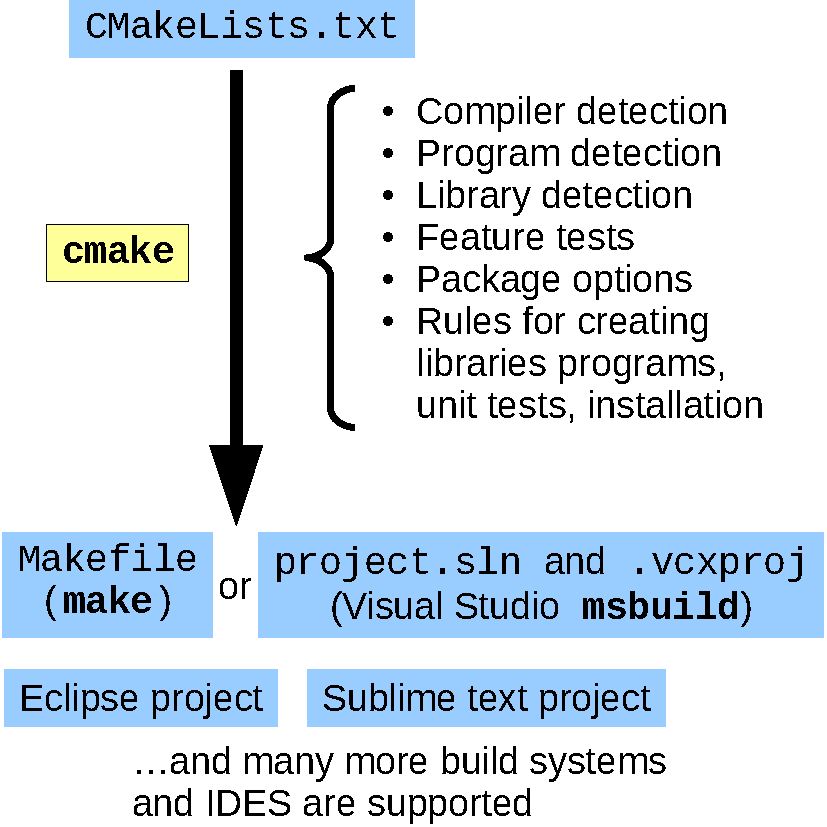
\includegraphics[width=0.65\textwidth]{cmake-flow}
\end{frame}

\begin{frame}
  \frametitle{Autotools overview}
  \centering
  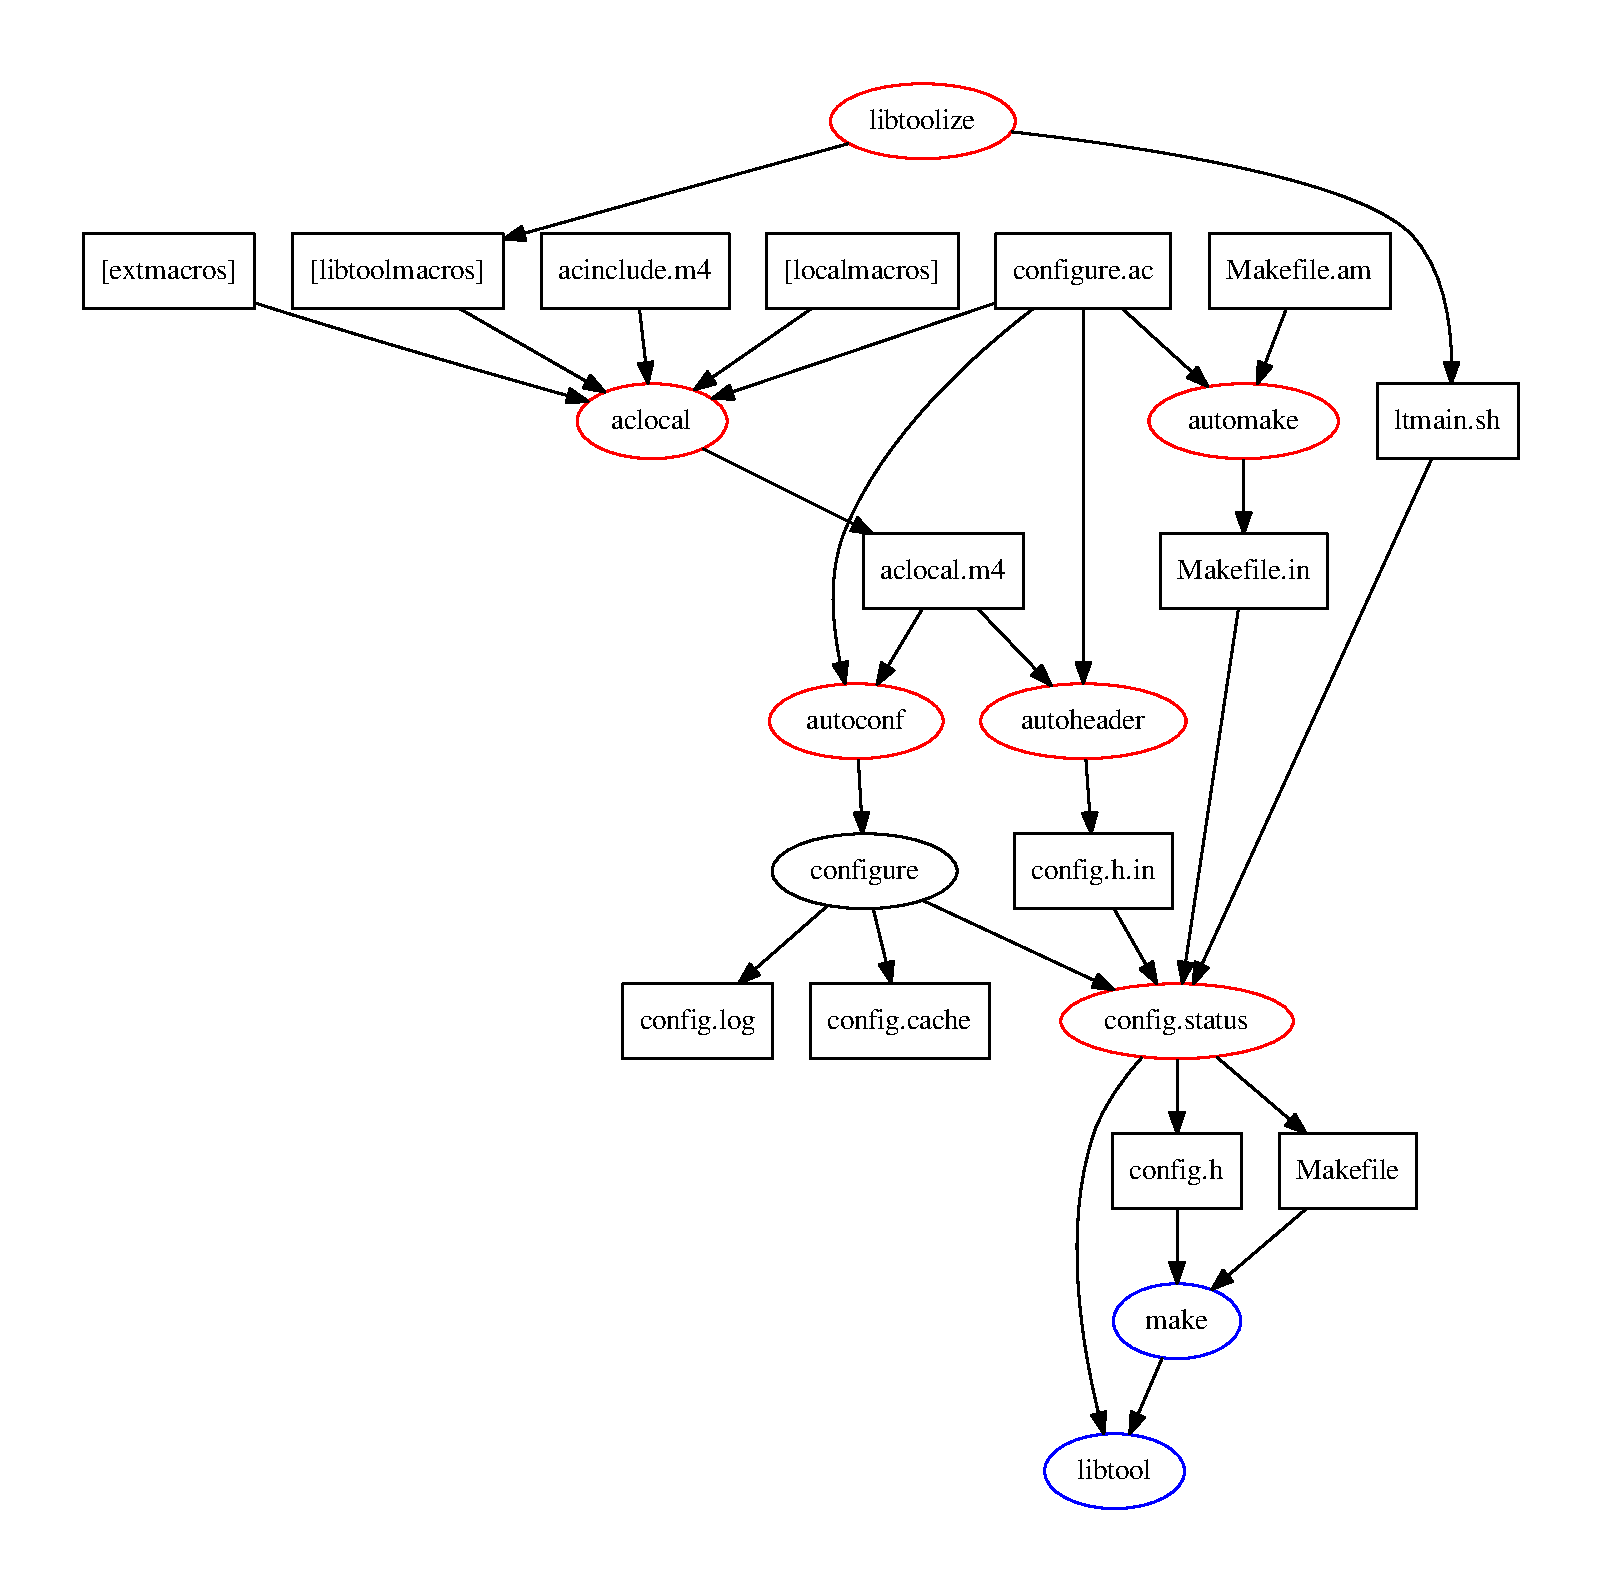
\includegraphics[width=0.78\textwidth]{autotools}
\end{frame}

\begin{frame}
  \frametitle{\cmd{cmake} overview}
  \medskip
  \centering
  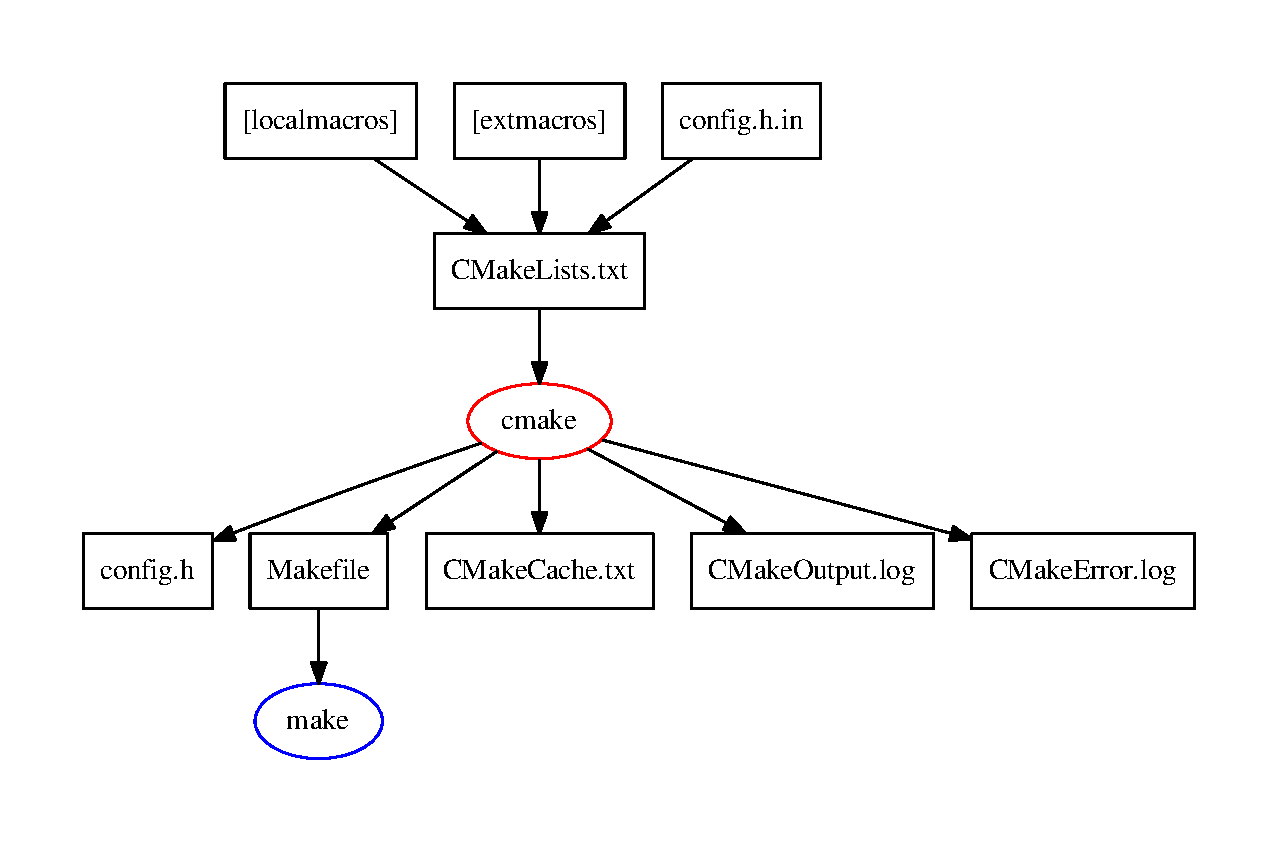
\includegraphics[width=\textwidth]{cmake}
\end{frame}

\section{cmake basics}

\subsection{Simple program}

\begin{frame}
  \frametitle{A simple program}

  \lstinputlisting{cmake-examples/program/CMakeLists.txt}

  \begin{itemize}
  \item Compiles \texttt{test.cpp} into the program \texttt{test-program}
  \end{itemize}

\end{frame}


\subsection{Simple library}

\begin{frame}
  \frametitle{A simple library}

  \lstinputlisting[firstline=8]{cmake-examples/library/CMakeLists.txt}

  \begin{itemize}
  \item Compiles \texttt{test.cpp} into the library \texttt{test-library}
  \item Adds ABI version number to \texttt{test-library}
  \item Compiles \texttt{main.cpp} into the program \texttt{test-program}
  \item Links \texttt{test-program} with \texttt{test-library}
  \end{itemize}
\end{frame}

\subsection{Language features}

\begin{frame}
  \frametitle{Variables, conditionals, loops}

  \lstinputlisting[firstline=3]{cmake-examples/control/CMakeLists.txt}

  \begin{itemize}
  \item Variables are lists of strings of 0, 1 or multiple values
  \end{itemize}
\end{frame}

\begin{frame}
  \frametitle{Feature tests}

  \lstinputlisting[firstline=5]{cmake-examples/feature/CMakeLists.txt}

  \begin{itemize}
  \item Feature tests probe system capabilities and adapt the build to the system
  \end{itemize}
\end{frame}

\begin{frame}
  \frametitle{Built-in feature tests}

  \lstinputlisting[firstline=5]{cmake-examples/feature2/CMakeLists.txt}

  \begin{itemize}
  \item CMake provides an extensive set of feature tests
  \item Custom feature tests can be written if needed
  \end{itemize}
\end{frame}


\appendix

\section[]{Acknowledgements}

\frame{
  \frametitle{Acknowledgements}
  \parbox[t]{0.45\textwidth}{
    \begin{itemize}
    \item OME Team, Dundee
      \begin{itemize}
      \item Jason Swedlow
      \item Jean-Marie Burel
      \item Mark Carroll
      \item Andrew Patterson
      \item …and the rest of the team
      \end{itemize}
    \end{itemize}
  }
  \parbox[t]{0.45\textwidth}{
    \begin{itemize}
    \item Micron, Oxford
      \begin{itemize}
      \item Douglas Russell
      \end{itemize}
    \item Glencoe Software
      \begin{itemize}
      \item Melissa Linkert
      \item Josh Moore
      \end{itemize}
    \end{itemize}
  }

  \begin{center}
    \vcenteredhbox{
\includegraphics[width=0.25\textwidth]{ome}} \hfill
    \vcenteredhbox{
\includegraphics[width=0.2\textwidth]{dundee}}\hfill
    \vcenteredhbox{
\includegraphics[width=0.5\textwidth]{wellcome}}
  \end{center}
}

\end{document}
